%!TEX encoding = UTF-8 Unicode
% !TeX spellcheck = en_GB
%%%%%%%%%%%%%%%%%%%%%%%%%%%%%%%%%%%%%%
\chapter{Experimental measurements of the Higgs boson }\label{chap:HiggsConstr}
%%%%%%%%%%%%%%%%%%%%%%%%%%%%%%%%%%%%%%
%In this chapter, I will discuss some of the bounds on the Higgs sector . Starting from an overview of the theoretical constraints on the Higgs potential, like the quantum triviality and unitarity. Then, the state-of-the-art experimental results on Higgs properties and couplings measurements will be discussed. However, despite many of the Higgs boson properties have been measured with good accuracy, there are still difficult observables in the Higgs sector and some open problems. These will be addressed at the end of this chapter.   
%%
The observation of the Higgs boson, then the extensive measurement of its properties and couplings has been on the top of the LHC programme priorities~\cite{ellis2000physics}. In the time this thesis was in the writing, the particle physics community will be celebrating a decade since the Higgs boson's discovery. Looking back 10 years ago, when I have witnessed the discovery of the Higgs boson via news press-conference in summer of 2012, and decided to be a part of this enormous step that humanity has taken, 
I feel astonished by the progress made in understanding this newly discovered particle!  \\ In this chapter, I will start by an overview of the extraordinary LHC and its experiments~in~\autoref{sec:theLHC}. Then, I will review the state-of-the-art status of experimental measurements of the Higgs properties in~\autoref{sec:Higgsprop}, cross-sections  and couplings in ~\autoref{sec:Higgscoupl}, and at the end I will discuss the challenges and outlook for the future runs of the LHC~\autoref{sec:Higgscouplchallenge}, of which the of the rest of this thesis is going to be aim address a small part of them.
\section{Overview of the Large Hadron Collider \label{sec:theLHC}}
\par The Large Hadron Collider~(LHC) is the largest particle accelerator in the CERN accelerators complex, with a circumference of about 26 \si{\kilo\metre},with over 9590 superconducting magnets cooled to 1.9 \si{\kelvin}. It was built as an upgrade to the  Large electron positron collider~(LEP) which ended its operation in the year 2000. The LHC contains four main experiments situated at the four beam collision points and detectors, and these experiments are: ATLAS, CMS, LHCb and ALICE, there also smaller experiments such as LHCf, MilliQan,TOTEM and others. For more details about the LHC cf.~\cite{cernfacts,welt-machine} or see the LHC technical design report~\cite{Bruning:2004ej} for more technical details.\\   The LHC started operation in September of 2008, with low energy proton beams, then gradually increased to an energy of 3.5 \TeV\ per proton to reach a centre of mass energy~$\sqrt{s}$ of 7 \TeV, and data-taking period started from 2011 . By 2012, its energy has increased to $\sqrt{s}= 8\ \TeV$ and operated at this energy for about year and half, then stopping in mid 2013 concluding what is known as \textbf{Run-I}. In 2015, the \textbf{Run-II} started with almost double the energy $\sqrt{s}= 13\ \TeV$, and lasted for ca. 3 years. As this thesis being written, preparations are being made to get \textbf{Run-III} started until 2024. During these runs, heavier nuclei such as $\prescript{207}{}{\mathbf{Pb}}$ and $\prescript{131}{}{\mathbf{Xe}}$ have been collided either with protons or with themselves~\cite{lhckomission}.  \\  From, 2025 and beyond, the \textbf{High-Luminosity} LHC~(HL-LHC) era will commence, see~\autoref{fig:lhcplan}.   Where the LHC will be shutdown for extensive upgrades ~\cite{Apollinari:2015bam} to potentially increase its energy to  $\sqrt{s}= 14\ \TeV$ and higher collision rates hence the term \emph{high luminosity}. Which leads us to an important notion in particle physics phenomenology ~\emph{integrated luminosity}.\\
\par The performance of colliders depends on many factors, but for phenomenological studies, like this thesis, one mainly considers the centre of mass energy $\sqrt{s}$ and the integrated luminosity~$\mathscr{L}$.
This is mainly due to the fact that particle colliders experiments are basically ``counting experiments'', and all of the bounds on physical observables or model parameters are obtained from the number of signal versus background events, and the number of expected events~$N_{expec}$ for a given resonance $R$ and a subsequent decay final state $X$ at any collider experiments is given by
\begin{equation}
	N_{expec} = \sigma(pp\to R) \, \mathcal B(R \to X)\,\mathscr{L}  \, \epsilon_{\mathrm{SEL}}.
\end{equation}
Here $ \epsilon_{\mathrm{SEL}}$ is the selection efficiency, which depends on many factors like the detector geometry and particle identification performance etc. , as well as the signal one searches for, it can be improved by better detected or selection cuts. The production cross-section increases typically with quadratically with $\sqrt {s}$, hence comes the need for higher energies but this can only achieved by building new colliders from scratch. The integrated luminosity can be increased much more easily, by longer running time of the same collider as it is the time integral of the collider's luminosity $L(t)$ over its operation time $T$
\begin{equation}
\mathscr{L} = \int^{T} L(t) .
\end{equation}
Therefore, we see that the integrated luminosity for the LHC experiments will increase over time, when more collisions taking place, as seen in figure~\autoref{fig:lumi} showing the integrated luminosity for ATLAS and CMS experiments. 
\begin{figure}[t!]
	\begin{center}
		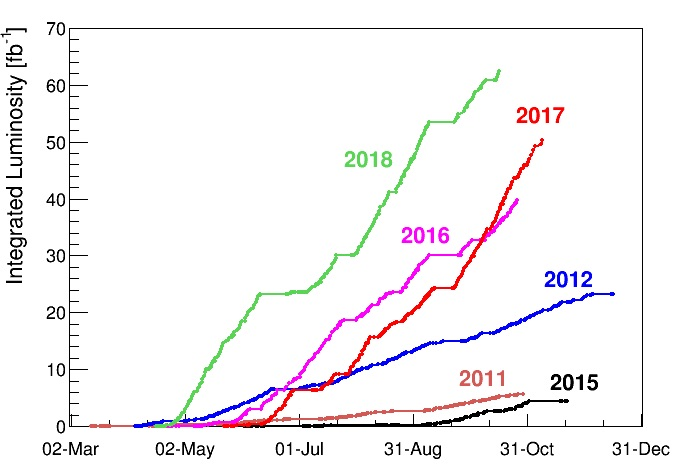
\includegraphics[width=8cm]{figures/lhc_lumi}
		\caption{The integrated luminosity of the CMS and ATLAS experiments combined over the period from 2011-2018, source~\cite{lhcpreformance}.  \label{fig:lumi} }
	\end{center}
\end{figure}
As thee protons travel in the LHC in \textbf{bunches}, and as these bunches cross, protons collide at a certain frequency $f$,  when two bunches with $N_1$ and $N_2$ protons per bunch, respectively. Each bunch will have an effective cross-section~$4 \pi \sigma_i$ corresponding to their physical sizes $\sigma \sim \SI{16}{\micro \meter}$, the luminosity is therefore given -approximately- by 
\begin{equation}
	L = \frac{f N_1 N_2}{4 \pi  \sigma_1 \sigma_2},
\end{equation}
which is for the LHC averages to about $ 10^{34}$ collisions \si{\per \centi\metre\squared \per \second}~\cite{closer,lhcpreformance}.  \\ The total physics-viable $pp$-collisions  integrated luminosity for Run-I was \SI{4.57}{\per \femtobarn} for \SI{7}{\tera\electronvolt} and \SI{20.3}{\per \femtobarn} for \SI{8}{\tera\electronvolt} (ATLAS~\cite{atlaslumi1}) and  \SI{5.55}{\per \femtobarn} at \SI{7}{\tera\electronvolt} and \SI{21.8}{\per \femtobarn} at \SI{8}{\tera\electronvolt} (CMS ~\cite{cmslumi}). As for Run-II the integrated luminosity is \SI{139}{\per \femtobarn} at \SI{13}{\tera\electronvolt } (ATLAS~\cite{atlaslumi2})  and \SI{137}{\per \femtobarn} at \SI{13}{\tera\electronvolt } (CMS ~\cite{cmslumi}). The expected integrated luminosity by the end of Run-III is  \SI{300}{\per \femtobarn}~\cite{Fartoukh:2790409} and \SI{3000}{\per \femtobarn} by the end of the HL-LHC at energy of \SI{14}{\tera\electronvolt }~\cite{Apollinari:2015bam}. 
%\begin{sidewaysfigure}[ht]
\begin{figure}[htbp!]
	\centering
		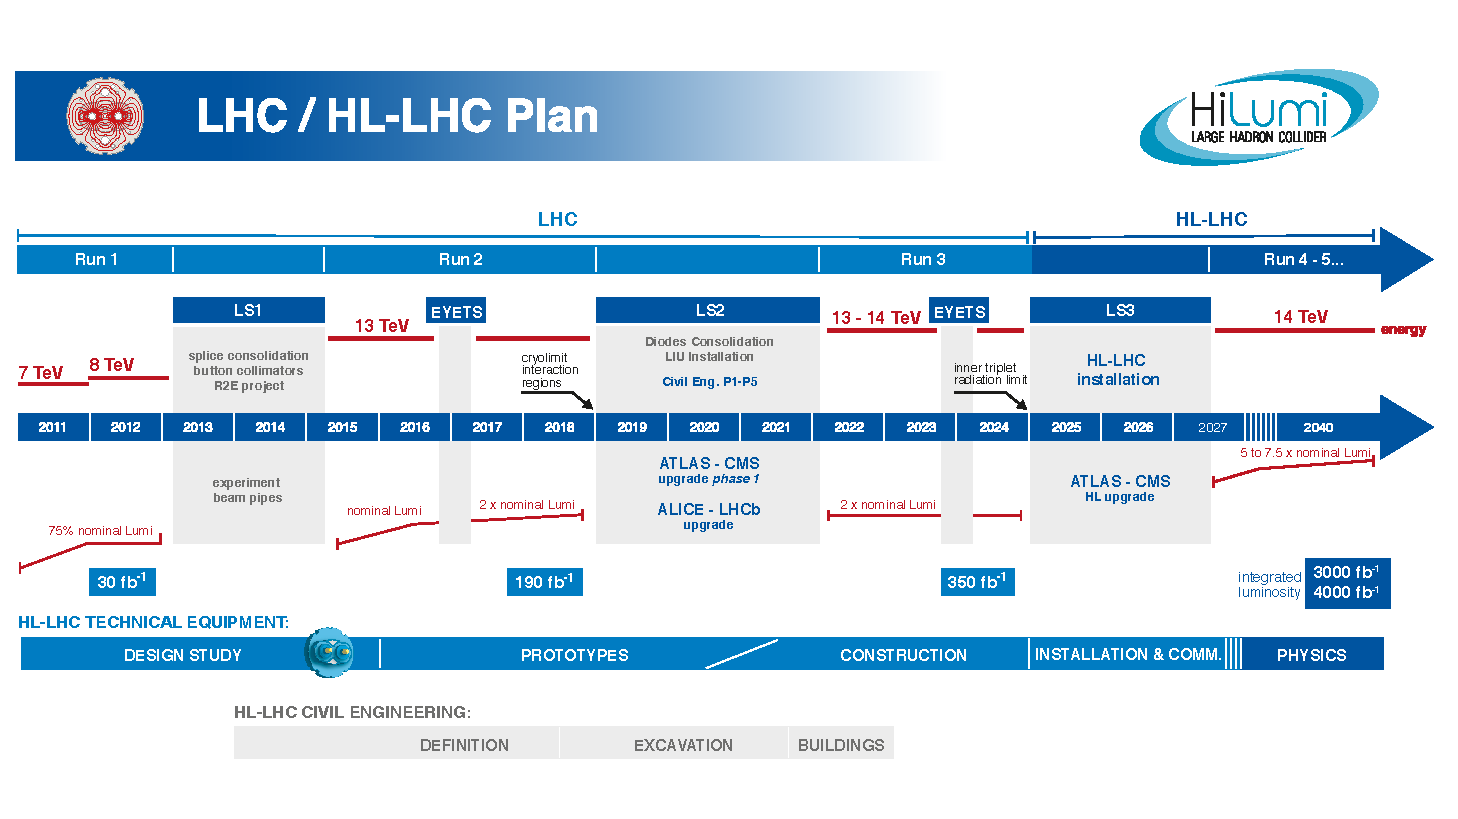
\includegraphics[width=\textwidth]{figures/HL-LHC-plan-2021-1}
	\caption{ A timeline of the LHC operation showing Run-I, Run-II and future planned runs of the LHC, including the HL-LHC, source~~\cite{lhckomission}. 
	}
\label{fig:lhcplan}
\end{figure}
%\end{sidewaysfigure}
%\FloatBarrier
\section{Higgs properties \label{sec:Higgsprop} }
\subsection{Higgs boson mass measurements}
In order to measure the mass of thee Higgs boson with high precision, one need to consider final states that can be reconstructed with high momentum and mass resolution, this is typically achieved when no hadronic constituents in the decays involved, such as  $ h \to \gamma \gamma$ and $ h \to Z Z^*\to 4 \ell$. Reconstructing the invariant mass distributions $m_{\gamma \gamma}$ and $m_{4\ell}$ one observes that the Higgs peak is narrow over a relatively smooth background, see~\autoref{fig:higgs_mass}, which is ideal for the measurement of the Higgs mass. It should be noted that the width of the resonance is due to the detector resolution and does not correspond to the actual Higgs width.\\
\begin{figure}[t!]
	\begin{center}
		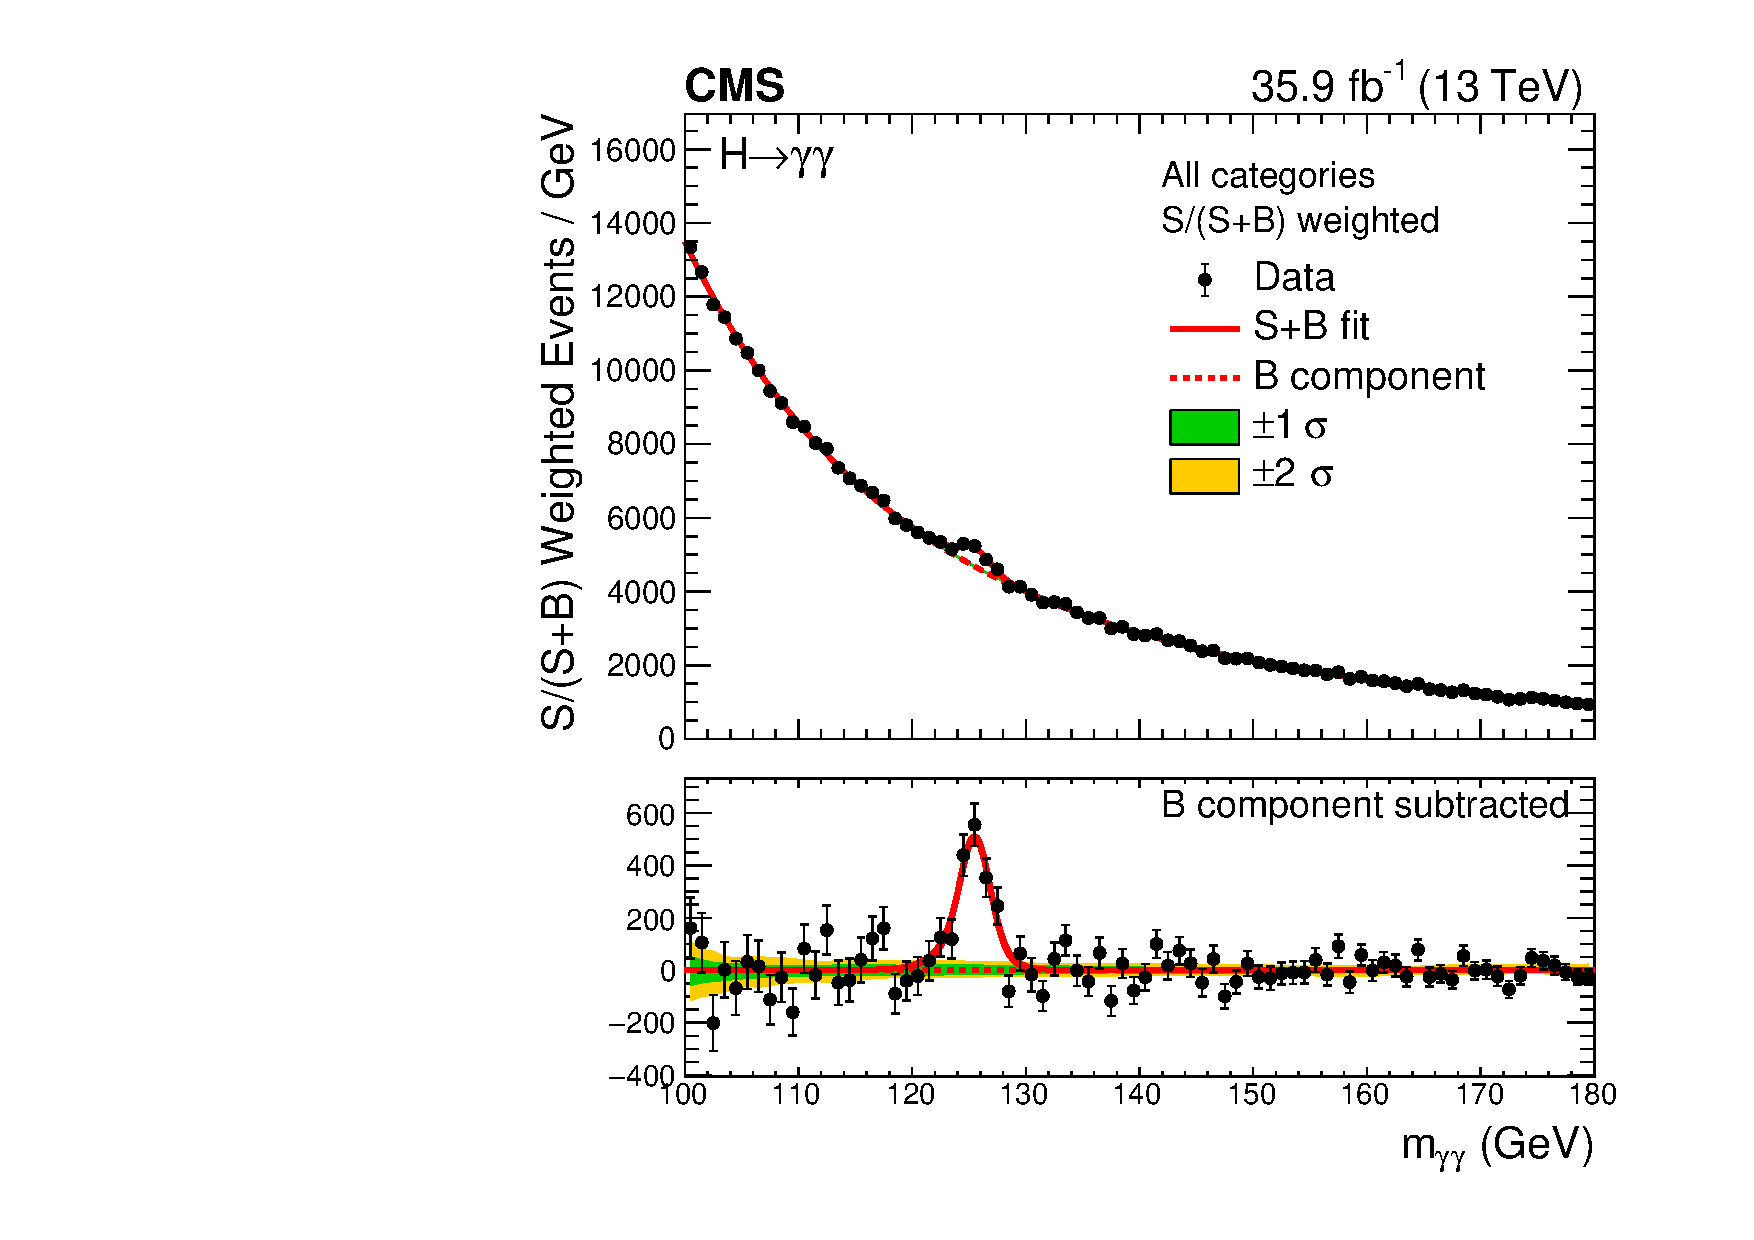
\includegraphics[width=0.45\textwidth]{figures/Higgs_results/CMS-HIG-19-004_Figure_005-b}
		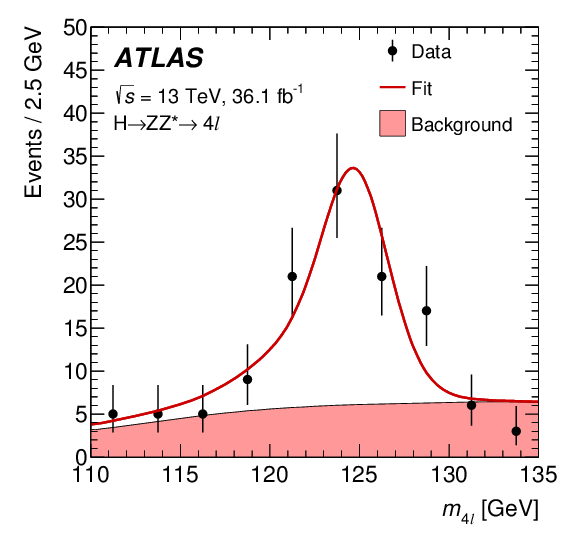
\includegraphics[width=0.45\textwidth]{figures/Higgs_results/dataAll_H4l_m4l_pdf_constrained} 
		\caption{The invariant mass distributions of diphoton~$m_{\gamma \gamma}$ (CMS~\cite{CMS:2020xrn}) and four lepton $m_{4 \ell}$ (ATLAS~\cite{ATLAS:2018tdk}) final states showing a clear peak at the Higgs mass, with smooth background. These final states are ideal for Higgs mass measurements. \label{fig:higgs_mass} }
	\end{center}
\end{figure}
There have been consistent improvements of the Higgs mass measurements since its discovery. In~\autoref{fig:meta_mass} I have preformed a meta analysis on ATLAS and CMS measurements of the Higgs mass in Run-I and Run-II of the LHC for both diphoton and $ZZ^*$ final states based on the data from the studies~\cite{ATLAS:2015yey,ATLAS:2018tdk,CMS:2017dib,CMS:2020xrn} using a random effects model~\cite{aronow_miller_2019}. The pooling of the studies yielded a mass measurement of $ m_h = 125.21 \pm 0.10$, which translates to a $0.11\%$ accuracy, the heterogeneity off the studies was found to be $I^2 =49\%$ ($p=0.05$) . Different measurements combination techniques were used in ~\cite{CMS:2020xrn} and ~\cite{Zyla:2020zbs} yielded different central values but all of the results agree within the uncertainties. 
\begin{figure}[h!]
	\begin{center}
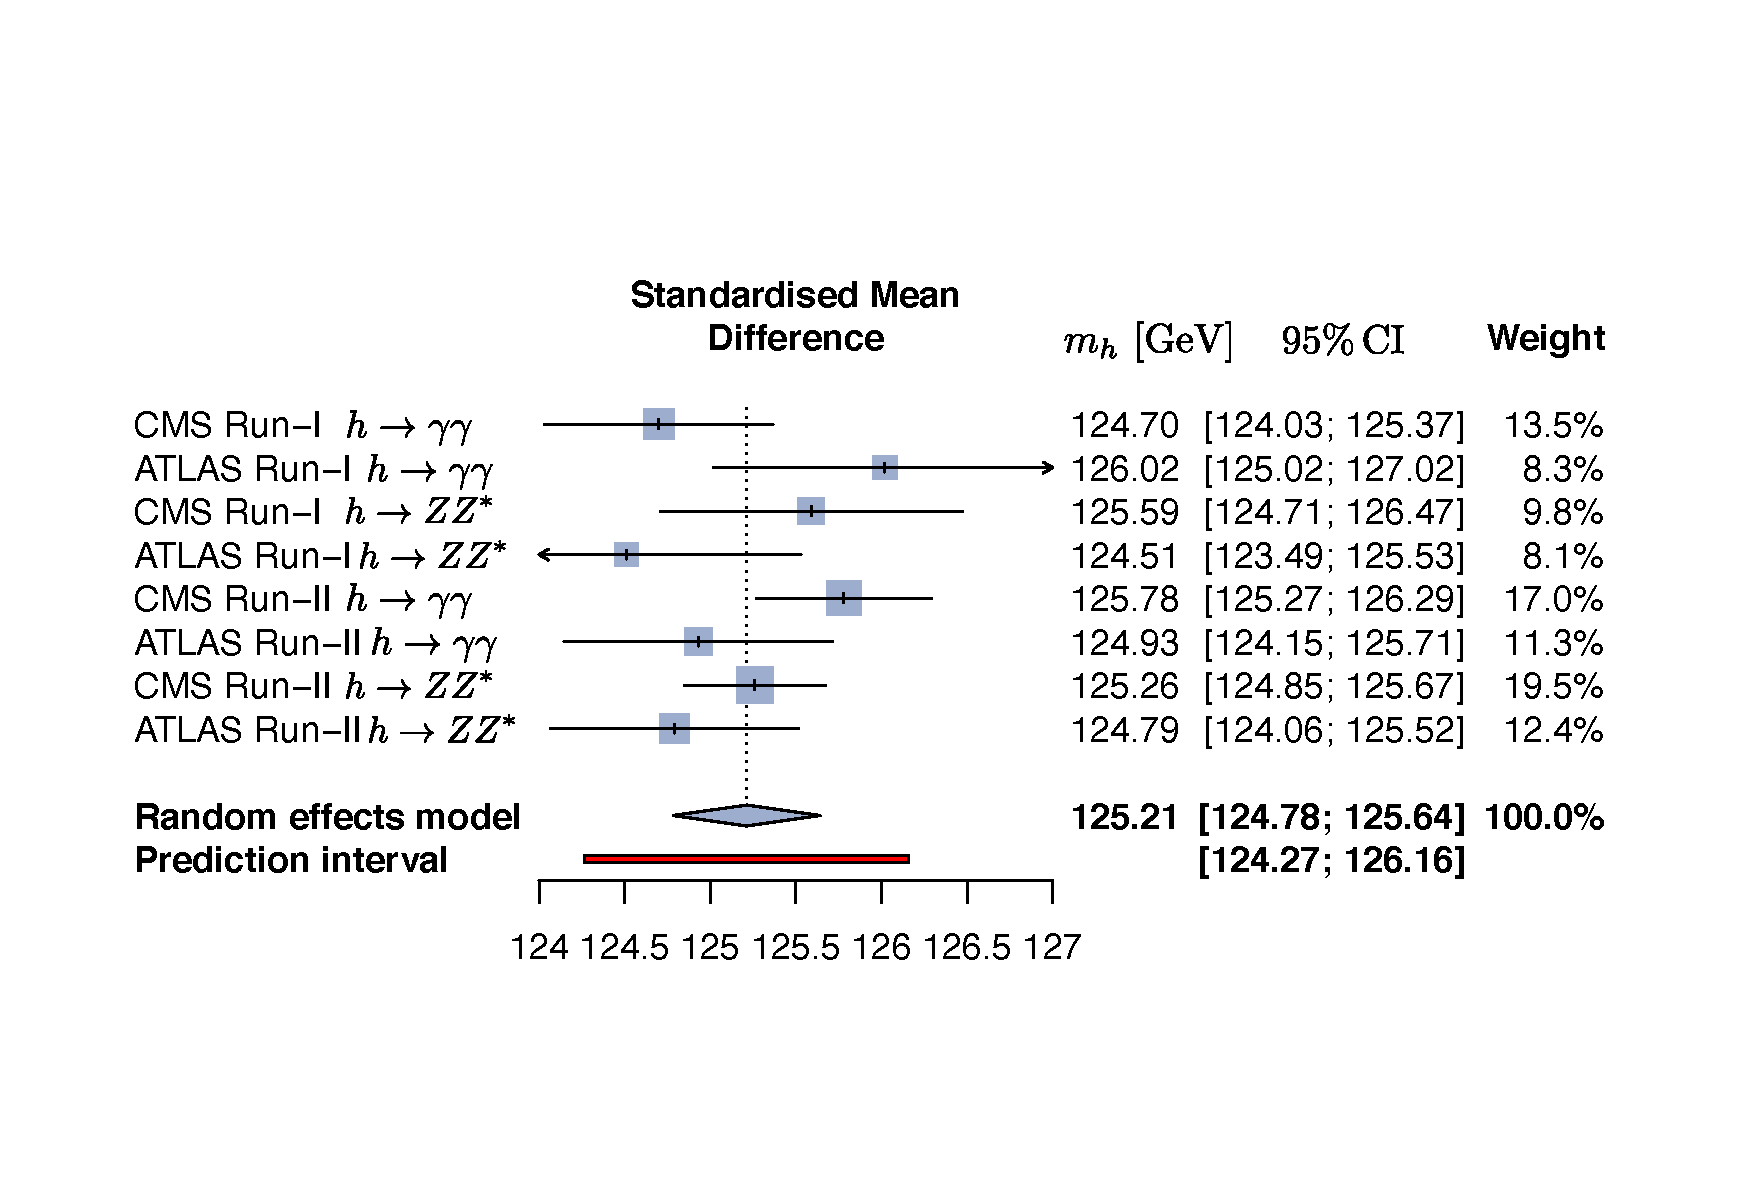
\includegraphics[width=1.\textwidth]{figures/foreest_pllot_higgs_mass}
		\caption{A meta analysis preformed to combine all the measurements of the Higgs mass from Run-I and Run-II, the combined result was obtained from pooling all of the studies using the random effects model method.\label{fig:meta_mass} }
	\end{center}
\end{figure}
\subsection{Higgs full width}
The SM values of the Higgs boson full width is ~$\Gamma_h=4.1$ \GeV\, and it can be accessed in the LHC by looking at the ratio of on-shell versus off-shell Higgs production and decay to the $ZZ^{(*)}$ state, and $ZZ^{(*)}\to 4 \ell, 2 \ell 2 \nu$, namely
\begin{equation}
\frac{\sigma(gg \to h\to Z Z^*)}{\sigma(gg \to h^*\to Z Z)} = \kappa_g^2 \kappa_Z^2 \frac{4 m_Z^2}{m_h \Gamma_h},
\label{widthform}
\end{equation}
where the $\kappa$ here denote the ratio between the measured/ or modified coupling with the Higgs and the SM prediction, i.e.
\begin{equation}
\kappa_X := \frac{g_{XX h}}{g_{XXh}^{\SM}}.
\label{kappa}
\end{equation}
Which is commonly used in reporting experimental constrains/ measurements of the Higgs couplings, as in the next section~\autoref{sec:Higgscoupl}. We shall discuss the $\kappa$ formalism more in~\autoref{chap:HiggsEFT}. \\ We see from~\eqref{widthform} that if one fixes the coupling between the gluons and the $Z$ boson and the Higgs it is possible to access the full width directly.  Unfortunately, it is not possible to directly measure the Higgs full width at the LHC, as this requires full reconstruction of the collision event and study the recoil mass which is only possible at lepton colliders~\cite{DeBlas:2019qco,Banerjee:2021huv}. 
Alas, it is still possible to extract bounds on $\Gamma_h$ using ~\eqref{widthform}. ATLAS used this method to constrain the full width of the Higgs using Run-II data~\cite{ATLAS:2018jym}, while CMS has preformed the same analysis using Run-I and Run-II data combined~\cite{CMS:2019ekd}, the results are 95\% CL bounds of $\Gamma_h$
\begin{align}
\Gamma_h &< \SI{14.4}{\giga\electronvolt} \,\,\,\, (\text{ATLAS}) & \SI{0.08}{\giga\electronvolt} <&\Gamma_h < \SI{9.16}{\giga\electronvolt}  \,\,\,\, (\text{CMS}),
\end{align}
with the combined bound being  $\sim 3 \Gamma_h^{\SM}$. 
\subsection{Higgs spin and parity \label{higgscp}}
As we have seen in ~\autoref{Higgsmech}, the Higgs boson in a scalar and $\mathcal{CP}$ even ($J^p= 0^+$) in the SM. However, the discovery of  a peak in the $m_\gamma \gamma$ distribution, would not automatically imply that the particle discovered is scalar, it could be a spin-$2$ boson, or a pseudoscalar  ($J^p= 0^-$). In order to study the $J^p$ properties of the Higgs, one needs to examine the differential distributions of angular variables such as rapidity~$y$ or transverse momentum~$\pt$. Both ATLAS and CMS collaborations studied using Run-I data the angular distributions of the Higgs decays $ h \to ZZ^*$, $h \to W W^*$ and $ h \to \gamma$, to study an anomalous $VVh$ coupling. Then test the alternative hypothesis for $J^p$ against the SM~\cite{ATLAS:2015zhl,CMS:2014nkk}.  The analysis results show that the SM ~$0^+$ hypothesis is favoured at $ >99.9\%$ CL. 
%\begin{figure}[htb!]
%	\begin{center}
%		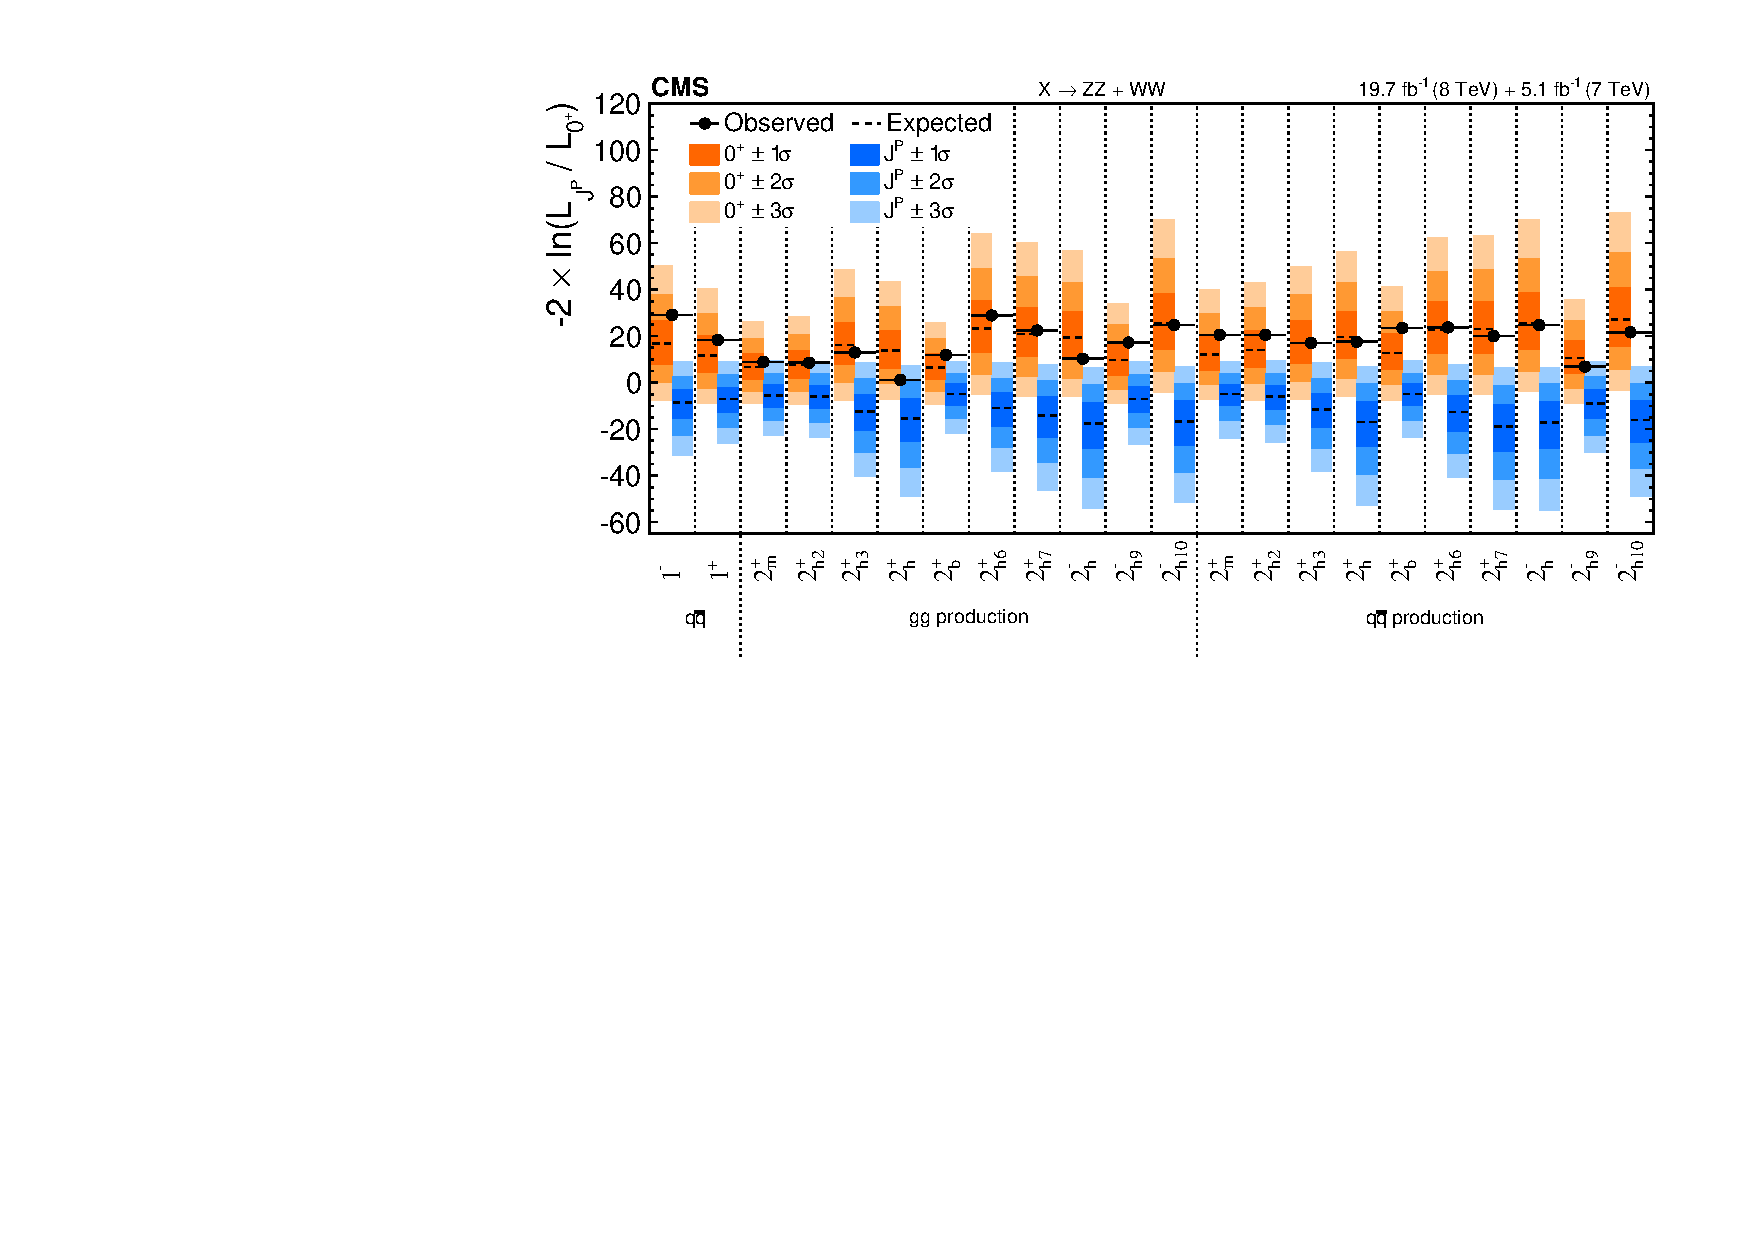
\includegraphics[width=1\textwidth]{figures/Higgs_results/CMS-HIG-14-018_Figure_018}
%		\caption{The test-statistic distributions for the SM Higgs hypothesis versus other $J^p$ hypothesises in the $x$ axis. The hypothesis testing was conducted using the  $ h \to ZZ^*$, $h \to W W^*$  final-states. The SM hypothesis is indicated in orange, while the alternatives are in blue. Measurements are indicated in black points. This plot is from the CMS collaboration~\cite{CMS:2014nkk}}	
%		\label{fig:jcphiggs}
%	\end{center}
%\end{figure}
\section{Measurements of Higgs rates and couplings \label{sec:Higgscoupl} }
\subsection{Higgs cross-sections}
\par The total inclusive Higgs cross-section has been measured using the the final states $ h \to \gamma \gamma$ and $ h\to Z Z^* \to 4 \ell$. and their combinations.  The measurements has been done at the three energies the LHC was operating at: 7 TeV, 8 TeV ~\cite{CMS:2015zpx} and 13 TeV~\cite{TheATLAScollaboration:2015uuh,CMS:2018gwt,CMS:2021ugl} and combined with more data and compared to the SM prediction as show in~\cite{ATLAS:2019mju}. As shown in~\autoref{fig:xstothiggs}, the measured inclusive cross-section is in agreement with the SM prediction across al of the LHC operation energies.
\begin{figure}[htb!]
	\begin{center}
		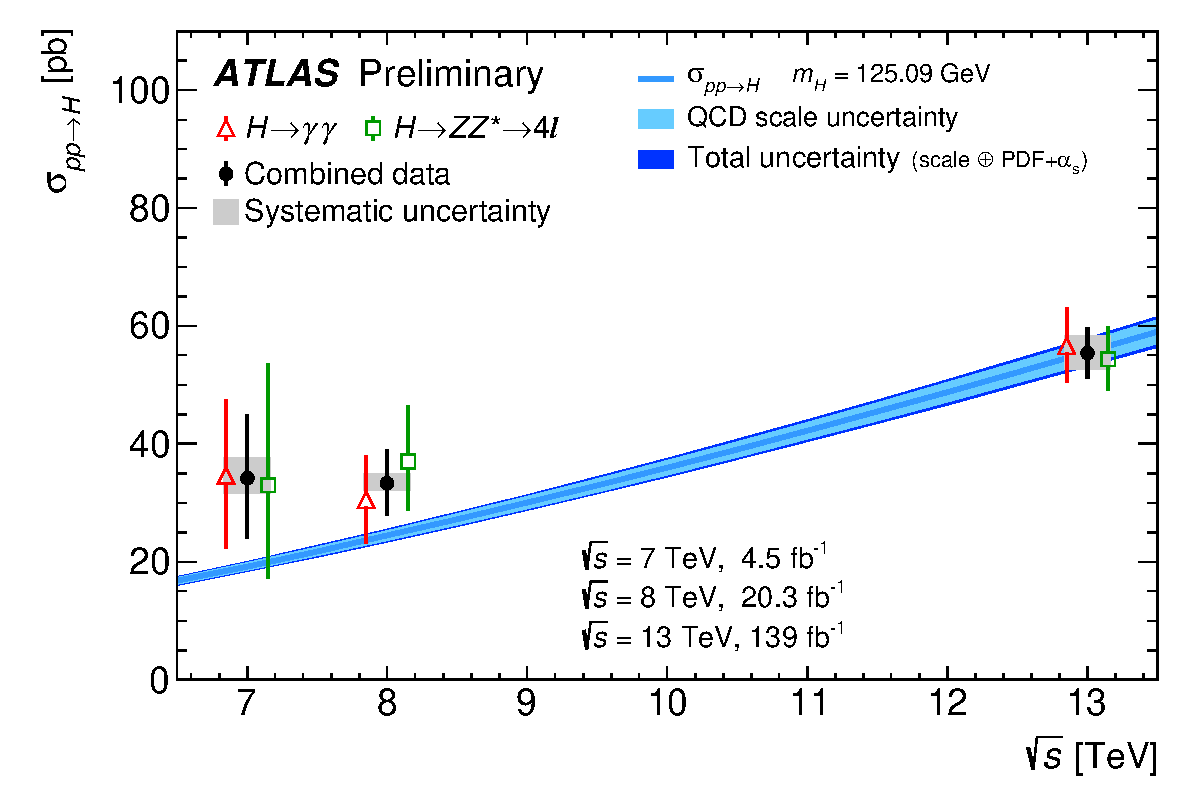
\includegraphics[height=0.35\textheight]{figures/Higgs_results/fig_01}
		\caption{The total inclusive cross-section measurements by ATLAS collaboration~\cite{ATLAS:2019mju} for $7$, $8$ and $13$ TeV using  $ h \to \gamma \gamma$ and $ h\to Z Z^* \to 4 \ell$. channels and their combination (black points) compared to the SM prediction with the  uncertainties shown as blue line with light and dark blue bands for QCD scale uncertainties and total uncertainties, respectively. }	
		\label{fig:xstothiggs}
	\end{center}
\end{figure}
%\FloatBarrier
\par In addition to the inclusive cross-section measurements,  differential cross-sections of the Higgs has been measured for $\pt$ and  $y$ as we have seen in~\autoref{higgscp} for Higgs's $J^p$ determination. Additional,  the differential cross-sections for other variables have been measured, and they include $N_{jets}, \pt^{jet}, m_{jj},\delta \phi_{jj]}$ and others using the channels $ h \to ZZ^*$, $h \to W W^*$ and $ h \to \gamma$. The most recent results using the full Run-II data can be found in Refs.~\cite{CMS:2018gwt,ATLAS:2019jst,ATLAS:2019mju,CMS:2019chr}.  
\par In addition to the total inclusive cross-section, a collection of measurements of Higgs production and decay rates has been carried out by both ATLAS and CMS. These measurements also carried out in , what is known as Standard Template Cross-Sections~(STXS) framework.The STXS's are fiducial cross-sections in exclusive phase-space regions or bins separately per Higgs boson production channel. They have the advantage of standardisation of cuts and final results such that measurements could be easily combined across analyses. More details about the STXS framework can be found in the reports of  LHC Higgs cross-sections working group~(LHCHXSWG) cf.~\cite{Berger:2019wnu}.  In~\autoref{table:resHiggsExp} I summarise the state-of-art measurements of the Higgs rates separated into production and decay channels using the total LHC Run-II data from ATLAS and CMS experiments. Additionally, I give the HL-LHC projections from CMS experiment as a comparison. The results in this table are written in terms of the signal strength, which is directly extracted from measuring the number of events dividing them by the standard model,
\begin{equation}
	\mu_{\mathrm{Exp}} := \frac{ \sigma \cdot \mathcal{B}}{ \sigma^{\SM} \cdot \mathcal{B}^{\SM}}.
\end{equation}
\newpage
\begingroup
\thispagestyle{plain}
\begin{table}[htb!]
\centering
\vspace{-1 cm}
 \footnotesize{ 
	{\renewcommand{\arraystretch}{0.75 }%
\begin{tabular}{clccc}
\toprule
\toprule
\multirow{5}{*}{ {\normalsize Production}}  &\multirow{5}{*}{ {\normalsize Decay}}&\multicolumn{2}{c}{ $\mu_{\mathrm{Exp}} \pm \delta \mu_{\mathrm{Exp}}$  (symmetrised)} &\multirow{5}{*}{ {\normalsize Ref.}} \\
%\cmidrule(r){3-4}
&   & { \bf     \scriptsize           LHC Run-II}&{ \bf  \scriptsize HL-LHC}&   \\
\cmidrule(r){3-4}
&   & { \scriptsize                   CMS $137 \, \mathrm{fb}^{-1} $}&  \multirow{2}{*}{CMS $3 \, \mathrm{ab}^{-1}$}&   \\
&   &  { \CG \scriptsize                   ATLAS $139 \, \mathrm{fb}^{-1} $} & &  \\
\midrule
\midrule
\multirow{ 13}{*}{ \normalsize ggF}         & \multirow{2}{*}{$h\to \gamma  \gamma$} & { \scriptsize                  $0.99 \pm 0.12$}& \multirow{2}{*}{$1.000\pm 0.042$}& \multirow{2}{*}{\cite{ATLAS:2020qdt,CMS:2021kom,CMS-PAS-FTR-18-011}}\\
                                           &                                                          &{ \scriptsize                   \CG $1.030 \pm 0.110$}&& \\ 
                                           \cmidrule(r){2-5}
                                           %%%%%%
                                    &  \mr{$h\to Z Z^*$}          & { \scriptsize                  $0.985 \pm 0.115$}&\multirow{2}{*}{$1.000 \pm 0.040$}&\multirow{7}{*}{\cite{ATLAS:2020qdt,CMS:2020gsy,CMS-PAS-FTR-18-011}}  \\
                                     &                                                      &{ \scriptsize                   \CG $0.945 \pm 0.105$}&& \\
                                     \cmidrule(r){2-4}
                                       %%%%%%
                                    &\mr{ $h\to W W^*$}         & { \scriptsize                  $1.285 \pm 0.195$} &\mr{ $1.000 \pm 0.037$} &\\
                                    & &                                            { \scriptsize                   \CG$1.085 \pm 0.185$} & &\\
                                                                         \cmidrule(r){2-4}
                                     %%%%%%
                                    &\mr{ $h\to \tau^+\tau^- $ }         & { \scriptsize                  $0.385 \pm 0.385$} &\mr{ $1.000 \pm 0.055$} &\\
                                 & &                                            { \scriptsize                   \CG$1.045 \pm 0.575$} & &\\
                                 \cmidrule(r){2-5}
                                 %%%%%%

                                  &\mr{ $h\to  b \bar b$  }      & { \scriptsize                 $2.54 \pm 2.44$} &\mr{ $1.000 \pm 0.247$} &\mr{\cite{CMS:2020gsy,CMS-PAS-FTR-18-011}}\\
                               & &                                            { \scriptsize                   \CG--} & &\\
                                 \cmidrule(r){2-5}
                               %%%%%%  %%%%%%   %%%%%%
                                  &\mr{ $h\to  \mu^+ \mu^-$  }      & { \scriptsize      $0.315 \pm 1.815$} &\mr{ $1.000 \pm 0.138$} &\mr{\cite{CMS:2020gsy,CMS-PAS-FTR-18-011} }\\
& &                                            { \scriptsize                   \CG--} & &\\
%%%%%%  %%%%%%   %%%%%%                               
\midrule
\midrule
%\crowcolor
\multirow{13}{*}{ \normalsize VBF}      
                                     %%%%%%
										&\mr{ $h\to \gamma  \gamma$ }         & { \scriptsize                  $1.175 \pm 0.335$ } &\mr{ $1.000 \pm 0.128$} & \mr{\cite{ATLAS:2020qdt,CMS:2021kom,CMS-PAS-FTR-18-011}}\\
										& &                                           { \scriptsize                   \CG$1.325 \pm 0.245$} & &\\
\cmidrule(r){2-5}
%%%%%%                                   
                                     &\mr{$h\to Z Z^*$ }         & { \scriptsize                  $0.62 \pm 0.41$ } &\mr{ $1.000 \pm 0.134$} & \multirow{7}{*}{\cite{ATLAS:2020qdt,CMS:2020gsy,CMS-PAS-FTR-18-011}}\\
                                    & &                                            { \scriptsize                   \CG$1.295 \pm 0.455$} & &\\
                                                                                             \cmidrule(r){2-4}
%%%%%%

                                   &\mr{$h\to W W^*$}         & { \scriptsize                  $0.65 \pm 0.63$ } &\mr{ $1.000 \pm 0.073$} & \\
                                    & &                                            { \scriptsize                   \CG$0.61 \pm 0.35$} & &\\
 \cmidrule(r){2-4}
%%%%%%0
                                   &\mr{$h\to \tau^+\tau^- $}         & { \scriptsize                  $1.055 \pm 0.295$ } &\mr{ $1.000 \pm 0.044$} & \\
& &                                            { \scriptsize                   \CG$1.17 \pm 0.55$} & &\\
\cmidrule(r){2-5}
%%%%%%0                                    
                                    &\mr{$h\to  b \bar b$}         & { \scriptsize                   -- } &\mr{--} & \mr{\cite{ATLAS:2020qdt} }\\
                                    & &                                            { \scriptsize                   \CG$3.055 \pm 1.645$} & &\\
                                    
                                  \cmidrule(r){2-5}
 %%%%%%  %%%%%%   %%%%%%
 &\mr{ $h\to  \mu^+ \mu^-$  }      & { \scriptsize               $3.325 \pm 8.075$} &\mr{ $1.000 \pm 0.540$} &\mr{ \cite{CMS-PAS-FTR-18-011}}\\
 & &                                            { \scriptsize                   \CG--} & & \\                                   
\midrule
\midrule
\multirow{10}{*}{ \normalsize  $t\bar t h$} 
%%%%%%0                                    
&\mr{ $h\to \gamma  \gamma$}         & { \scriptsize                $1.43 \pm 0.30$ } &\mr{$1.000 \pm 0.094$} & \mr{ \cite{ATLAS:2020qdt,CMS:2021kom,CMS-PAS-FTR-18-011} }\\
& &                                            { \scriptsize                   \CG$0.915 \pm 0.255$} & &\\

\cmidrule(r){2-5}

                                    
%%%%%%0                                    
&\multirow{3}{*} { $h\to V V^*$   }         & { \scriptsize              $0.64 \pm 0.64$({\color{Mahogany}$ZZ^*$}) } &{ \scriptsize   $1.000 \pm 0.246$ ({\color{Mahogany}$ZZ^*$}) } & \multirow{8}{*}{\cite{ATLAS:2020qdt,CMS:2020gsy,CMS-PAS-FTR-18-011}}  \\
& &                                            { \scriptsize                   $0.945\pm 0.465$ ({\color{Mahogany} $W W^*$})} & { \scriptsize   $1.000 \pm 0.097$ ({\color{Mahogany} $W W^*$})} &\\
& &                                            { \scriptsize                   \CG $1.735 \pm 0.545$} & { \scriptsize   --}&\\
\cmidrule(r){2-4}                                    

&\mr{$h\to \tau^+\tau^- $}         & { \scriptsize                $0.845 \pm 0.705$} &\mr{ $1.000 \pm 0.149$} & \\
& &                                            { \scriptsize                   \CG $1.27 \pm 1.0$} & &\\
\cmidrule(r){2-4}                                    

&\mr{ $h\to  b \bar b$  }         & { \scriptsize                 $1.145 \pm 0.315$} &\mr{ $1.000 \pm 0.116$} & \\
& &                                            { \scriptsize                   \CG $0.795 \pm 0.595$} & &\\                                                        
\midrule
\midrule
\multirow{9}{*}{ \normalsize $Vh$}        

                      
&\mr{ $h\to \gamma  \gamma$  }         & { \scriptsize   $0.725 \pm 0.295$ } &{ \scriptsize   $1.000 \pm 0.233$ ({\color{Mahogany}$Zh$}) } & \multirow{2}{*}{ \cite{ATLAS:2020qdt,CMS:2021kom,CMS-PAS-FTR-18-011}  }  \\
& &                                            { \scriptsize                   \CG $1.335 \pm 0.315$} & { \scriptsize   $1.000 \pm 0.139$ ({\color{Mahogany} $W^\pm h$})} &\\
\cmidrule(r){2-5}           
%%%%%%0              
                                    
&\mr{ $h\to Z Z^*$    }         & { \scriptsize   $1.21 \pm 0.85$ } &{ \scriptsize   $1.000 \pm 0.786$ ({\color{Mahogany}$Zh$}) } & \multirow{2}{*}{ \cite{ATLAS:2020qdt,CMS:2020gsy,CMS-PAS-FTR-18-011}  }  \\
& &                                            { \scriptsize                   \CG $1.635 \pm 1.025$} & { \scriptsize   $1.000 \pm 0.478$ ({\color{Mahogany} $W^\pm h$})} &\\
\cmidrule(r){2-5}           
%%%%%%0                                         
                                  
 &\mr{ $h\to W W^*$    }         & { \scriptsize   $1.850\pm 0.438$ } &{ \scriptsize   $1.000 \pm 0.184$ ({\color{Mahogany}$Zh$}) } & \multirow{2}{*}{  \cite{CMS:2021ixs,CMS-PAS-FTR-18-011} }  \\
 & &                                            { \scriptsize                   \CG --} & { \scriptsize   $1.000 \pm 0.138$ ({\color{Mahogany} $W^\pm h$})} &\\
 \cmidrule(r){2-5}           
 %%%%%%0                                                                                                            
 &\mr{$h\to  b \bar b$      }         & { \scriptsize  -- } &{ \scriptsize   $1.000 \pm 0.065$ ({\color{Mahogany}$Zh$}) } & \multirow{2}{*}{  \cite{ATLAS:2020qdt,CMS-PAS-FTR-18-011} }  \\
& &                                            { \scriptsize                   \CG $1.025 \pm 0.175$} & { \scriptsize   $1.000 \pm 0.094$ ({\color{Mahogany} $W^\pm h$})} &\\

%%%%%%0                                        
                                    
\midrule
\midrule
\multirow{2}{*}{ \normalsize $Zh$ { \scriptsize {\color{Mahogany} CMS     }   }}    & $h\to \tau^+\tau^- $ & $1.645 \pm 1.485$&\multirow{5}{*}{--} &\multirow{5}{*}{ \cite{CMS:2020gsy} }  \\
& $h\to  b \bar b$       &$0.94 \pm 0.32$&&\\                         
 \cmidrule(r){2-3}    
\multirow{2}{*}{ \normalsize $W^\pm h${ \scriptsize {\color{Mahogany} CMS     }   }}           & $h\to \tau^+\tau^- $ &$3.08 \pm 1.58$&&\\
& $h\to  b \bar b$      & $1.28 \pm 0.41$&&\\                  
\midrule
\midrule
\end{tabular}
}
}
\caption{The experimental single Higgs production and decay rates measurements from the  complete  data of LHC Run II and projections for the HL-LHC. The uncertainties were symmetrised here. The table is published in~\cite{Alasfar:2022zyr}.  }
\label{table:resHiggsExp}
\end{table} 
\endgroup
\FloatBarrier
\subsection{Constraints on Higgs couplings}
The measurements of the Higgs rates and their combination (also including STXS) have been used to set bounds on the Higgs couplings, the most recent bounds - as this thesis being written - have been reported by ATLAS using the Higgs inclusive rates and STXS for the full Run-II data~\cite{ATLAS2021vrm}, and  by CMS using Higgs rates shown in ~\autoref{table:resHiggsExp} ~\cite{CMS:2020gsy}. In~\autoref{fig:couplings-bound}, I present the aggregation the ATLAS and CMS bounds on the Higgs coupling modifiers in the $\kappa$ formalism defined in eq.~\eqref{kappa}. The aggregation of these bounds was preformed using the method described in~\cite{BHHR} assuming there is no correlation between ATLAS and CMS measurements.  
\begin{figure}[htb!]
	\begin{center}
		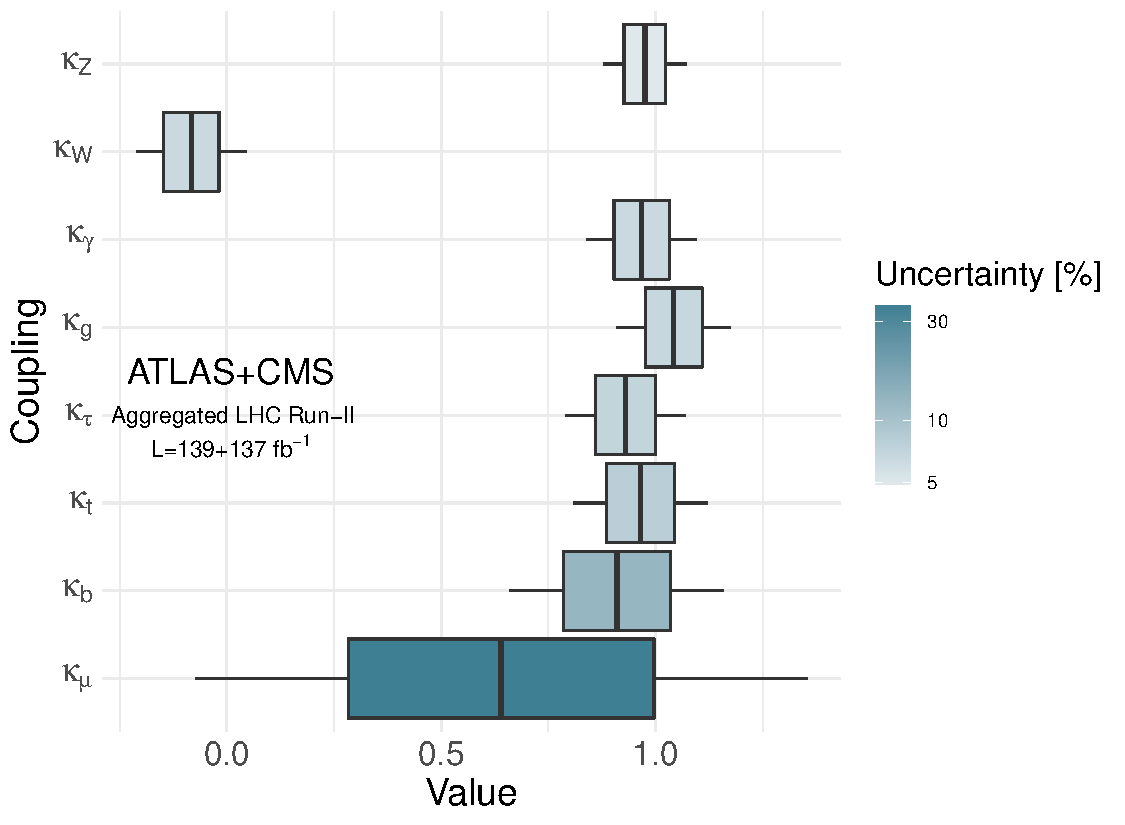
\includegraphics[height=0.3\textheight]{figures/agg_higgs_couplings}
		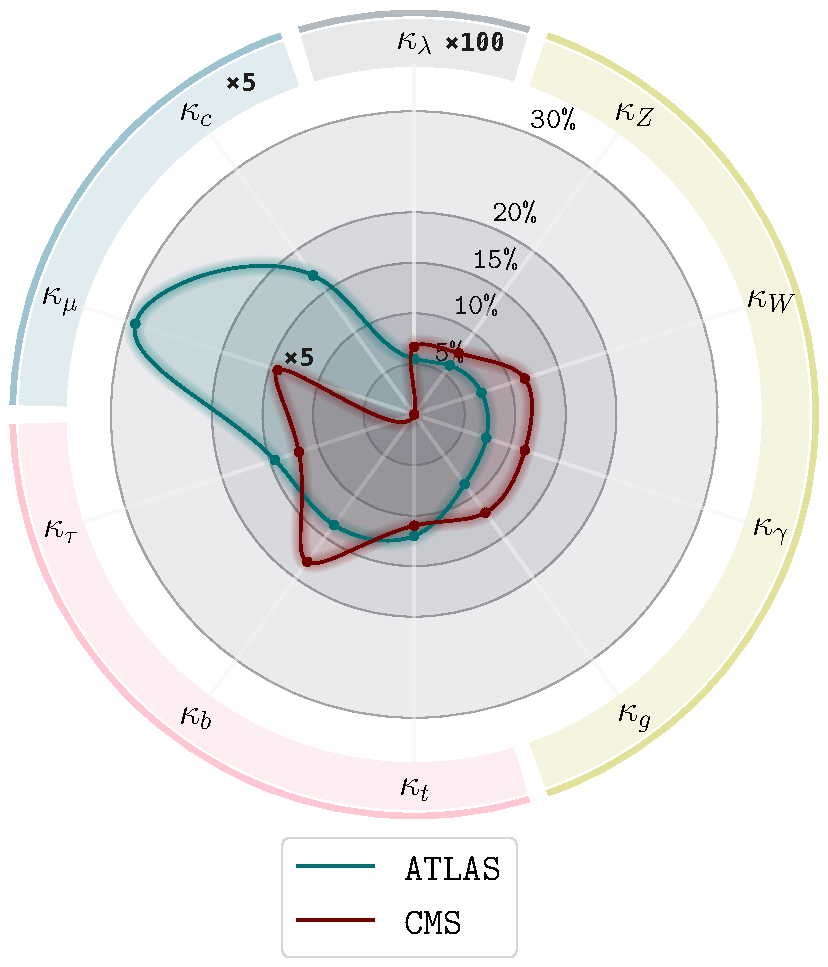
\includegraphics[height=0.3\textheight]{figures/Higgs_couplings_poster}
		\caption{Meta analysis aggravating the most recent bounds from ATLAS~\cite{ATLAS2021vrm} and CMS~\cite{CMS:2020gsy} on the Higgs couplings modifiers $\kappa$. \la{update the fig}  }	
		\label{fig:couplings-bound}
	\end{center}
\end{figure}
\par Examining~\autoref{fig:couplings-bound}, we observe that the bounds on the Higgs boson's coupling to the gauge boson, including the effective couplings to $\gamma$ and $g$, as well as the couplings to the third-generation fermions are in few percent within the SM prediction. The bounds on the coupling to the $W$ boson seems to favour a negative value in CMS fits, due to the channel used to constraint it $ h \to WW$ which depends on $ \kappa_W^2$, thus making the best fit value of $ \sim -1$ within the SM prediction. An independent analysis on the relative signs of $\kappa_W$ and $\kappa_t$ was preformed using $th/t \bar{t} h$ processes in Ref.~\cite{CMS:2018jeh}, hence only the absolute value of $\kappa_W$ is reported in my combination of the analysis results.  Additionally,  the observation of the decays $ h \to b \bar{b}$~\cite{CMS:2018nsn,ATLAS:2018kot,ATLAS:2019yhn} and $h \to \tau \tau$~\cite{ATLAS:2018ynr,CMS:2019pyn} leading to direct measurements of the beauty and $\tau$ Yukawa couplings has  made their bounds comparable to the gauge bosons and top couplings with the Higgs, having less than $10\%$ uncertainty.  Au contraire, bounds on the Yukawa couplings of second and first generation fermions remain very weak.  
\par Recently, searches for the decay  $ h\to \mu \mu$~\cite{ATLAS:2020fzp,CMS:2020xwi} using the whole Run-II data by both collaborations, yielded an evidence fr its observation of about $ 3 \sigma$. Improving the constraints on $\kappa_\mu$, though as seen in ~\autoref{fig:couplings-bound}, the uncertainty remains high $ \sim 36 \%$.  Searches for the Higgs decaying to charm pairs is significantly more challenging than the dimuon decays and only yielded an upper 95\% CL  bounds on $ |\kappa_c|$ of $8.5$ for ATLAS~\cite{ATLAS-CONF-2021-021} and $70$ for CMS~\cite{CMS:2019hve}. There is no planned direct searches for the first generation Yukawa couplings (\emph{direct}) measurements planned for the LHC as it is not possible to directly access decays of the Higgs to up or down quarks. Other methods for probing these couplings will be extensively discussed in  ~\autoref{chap:MLLightYuk}.
\par By the end of the HL-LHC, it is projected that the couplings of the Higgs, including the couplings with gauge bosons, third generation fermions as well as the muon Yukawa will be measured at few percent level, particularly the couplings with the gauge bosons will be reaching $ \sim 1\%$ level uncertainty~\cite{Bernius:2666331}. This is highlighted by~\autoref{fig:couplings-hlhlc}, this figure shows the improvement in the $\kappa$ measurement uncertainty expected by the HL-LHC over Run-II.
\begin{figure}[htb!]
	\begin{center}
		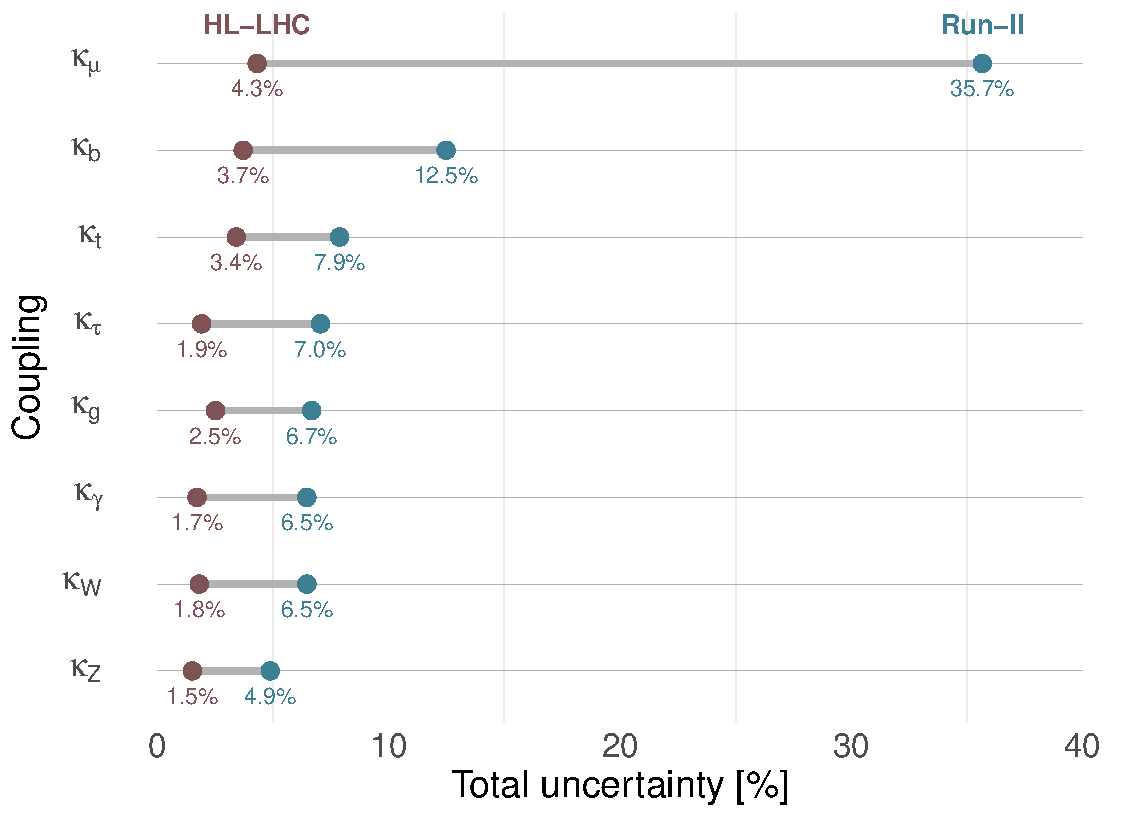
\includegraphics[height=0.35\textheight]{figures/run2-hl-dumble}
		\caption{ \textit{How much the HL-LHC is projected to improve Higgs couplings' measurement?}  The combining ATLAS and CMS projections }	
		\label{fig:couplings-hlhlc}
	\end{center}
\end{figure}
%\subsection{Miscellaneous Higgs measurements }

\section{Challenges and outlook \label{sec:Higgscouplchallenge} }
\par The future runs of the LHC  hold a lot of potential for further understanding of the 10-year old Higgs boson ! Although, for some processes and couplings there will still be a lot of challenges. For instance, the observation of $h \to c \bar{c}$ will require highly efficient charm-tagging, which is expected to improve at the HL-LHC by a factor of 2.5~\cite{ATL-PHYS-PUB-2018-016}.  The signal strength with rare decay $ h \to Z \gamma$ currently is constrained to $3.6$ times the SM values at 95\% CL ~\cite{ATLAS:2020qcv} and it is projected to be measured at the HL-LHC with~$\sim 10\%$ uncertainty. 
\par One of the couplings of the Higgs which we did not discuss above is the Higgs self-interaction (trilinear and quartic), as I have shown in~\autoref{pwusection} that the perturbative unitarity bound derived in Ref.~\cite{DiLuzio:2017tfn}  is the strongest bound on these couplings so far. This is due to the fact that to experimentally measure the Higgs self-coupling, one needs to search for double Higgs  production to access the trilinear self-coupling, and triple Higgs production for the quartic. These processes are very challenging, due to their low inclusive cross-section $\sim 30$ fb for~$hh$~\cite{Dawson:1998py} and $<0.1$ fb for $hhh$ at LHC maximum expected operational energy of $14$ TeV and the latter is challenging even for future colliders of inclusive cross section at $100$ TeV of only $\sim 5$ fb~\cite{Papaefstathiou:2015paa}; as opposed to single Higgs production with inclusive cross-section of $\sim 70$ pb. Certainly the difficulty is aggrivated when one considers that the second Higgs would also decay, further lowering the signal strength. The triple Higgs production thus, will not be accessable at the LHC and consequently the quartic self-coupling. However, there is a lot of potential for the trilinear self-coupling, particularly at the HL-LHC. 
\par In ~\autoref{chap:4topSingleHiggs} I will discuss the potential for using single Higgs processes as proposed by several studies, cf.~ \cite{McCullough:2013rea, Gorbahn:2016uoy, Degrassi:2016wml, Bizon:2016wgr, Maltoni:2017ims, Degrassi:2019yix, Degrassi:2021uik, Haisch:2021hvy} and the challenges accompanying it. Later in~\autoref{chap:overviewDiHiggs} the Higgs pair production at the LHC will be overviewed along the current and future searches for this process and the bounds from them on the trilinear Higgs self-coupling. 
\par Another elusive couplings that we have came across are the light Yukawas. In particular light quark Yukawa couplings of the first generation. After overviewing the proposed methods for constraining them, in~\autoref{chap:lightyuk} I will discuss a novel method for directly measuring light quark Yukawa coupling using Higgs pair production. And in~\autoref{chap:MLLightYuk} a sophisticated method based on interpretable machine learning will be showcased, by which, it is possible to simultaneously constrain the two elusive Higgs interactions: light Yukawas and the trilinear self-coupling using Higgs pair production !
